%! program = pdflatex

%\documentclass[12pt,a4paper]{memoir} % for a long document
\documentclass[12pt,a4paper,article]{report} % for a short document
\usepackage[spanish]{babel}

\title{Programa de física de neutrinos de Euskadi: Memoria científica 2024}
%\author{J.J. Gómez-Cadenas, F. Monrabal, F. L\'opez-Gejo \\ Donostia International Physics Center}
\date{} % Delete this line to display the current date
\usepackage{tcolorbox}
\usepackage{amsmath}
\usepackage[official]{eurosym}
\usepackage{xcolor}
\usepackage{makecell}



%%%Adjusting space between paragraphs
\setlength{\parskip}{12pt}

%%%%Hyphenation
 \hyphenation{TEK-NI-KER}
\def\coess{{\bf CoESS}}
\def\xess{{\bf XeESS}}
\def\gess{{\bf GeESS}}
\def\cess{{\bf CsIESS}}
\def\xed{{\bf XeDemo}}
\def\ged{{\bf GeHP1}}
\def\ced{{\bf CsIDemo}}
\def\gap{{\bf GaP}}
\def\crysp{{\bf CrysP}}
\def\ness{{\bf nESS}}
%%% BEGIN DOCUMENT
\begin{document}

\maketitle
%\tableofcontents* % the asterisk means that the contents itself isn't put into the ToC
\begin{centering}
\section*{Introducción}
\end{centering}
%\section{}
%\subsection{}

El programa de de física de neutrinos de Euskadi, en el que participan varios centros de excelencia del País Vasco (DIPC, CFM, UPV/EHU)  propone destacadas contributions a varios experimentos de neutrinos de primera talla mundial. 

En concreto, nuestros grupos lideran varias tecnología punteras para detectar dispersión coherente de neutrinos, lo que nos permite proponer experimentos de alta precisión en varias fuentes de neutrinos diferentes. Durante los últimos años, nos hemos focalizado en la Fuente Europea de Espalación de neutrones (European Spallation Source, ESS). La ESS, cuya puesta en marcha está prevista para 2026/2027, tiene el potencial de convertirse en una de las fuentes de neutrinos más importantes del mundo. Sin embargo, los retrasos en la puesta en marcha de esta facilidad, nos ha llevado a explorar otras posibilidades, en concreto, la posibilidad de realizar experimentos en la fuente de neutrones de JPARC, en Japón. Nuestro grupo ha propuesto programas experimentales a ambas facilidades. Hay que resaltar que se trata de programas compatibles, dado el considerable retraso de la ESS.  Por último, pero no por ello menos importante, estamos realizando un experimento de medida del flujo de neutrinos (usando dispersión elástica coherente) en la central nuclear de Vandellós

Por otra parte, Euskadi lidera el experimento NEXT que busca demostrar que el neutrino es su propia antipartícula en el Laboratorio Subterráneo de Canfranc (LSC) y en particular, la colaboración entre el DIPC el CFM y la UPV/EHU lidera el programa BOLD, que busca detectar el dicatión de Ba$^{2+}$ producido en la desintegración doble beta del ${}^{136}$Xe. 

Finalmente, el DIPC juega un importante papel en la colaboración Hyper-Kamiokande, que está construyendo en la actualidad un detector de medio millón de toneladas, que supondrá un auténtico observatorio de neutrinos, con un rico programa de física que abarca desde el estudio de oscilación de neutrinos hasta la observación de Supernovas.

Además de nuestra extensa participación en experimentos de física fundamental, el programa de física de neutrinos de Euskadi está desarrollando aplicaciones a la sociedad de nuestras tecnologías, que, en concreto, han llevado a CRYSP, un proyecto que propone desarrollar un scanner PET de cuerpo completo basado en cristales monolíticos de Yoduro de Cesio operando a temperaturas criogénicas.



\section*{Los programas experimentales de física de neutrinos}

En esta sección ofrecemos un conciso resumen de los programas experimentales en marcha en Euskadi. 

\subsection*{NEXT}

\begin{figure}[bht!]
\begin{center}
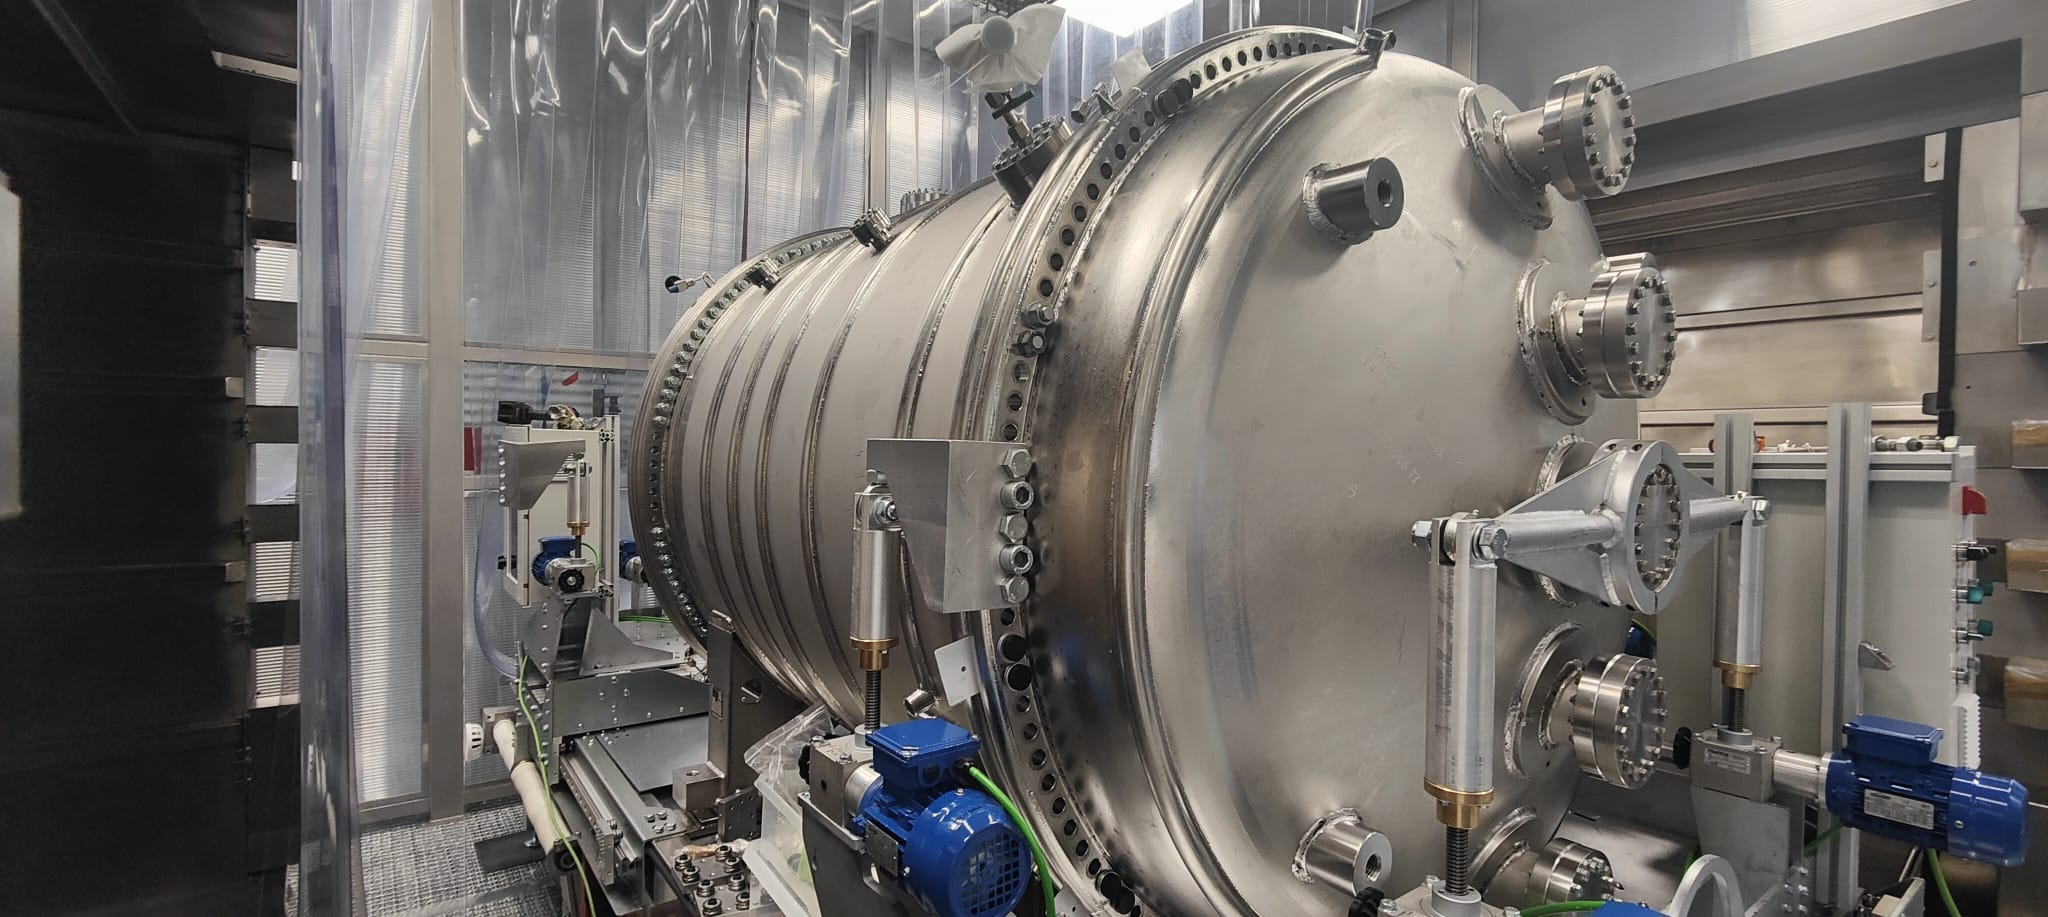
\includegraphics[width=8cm]{img/next100-vessel.jpeg}
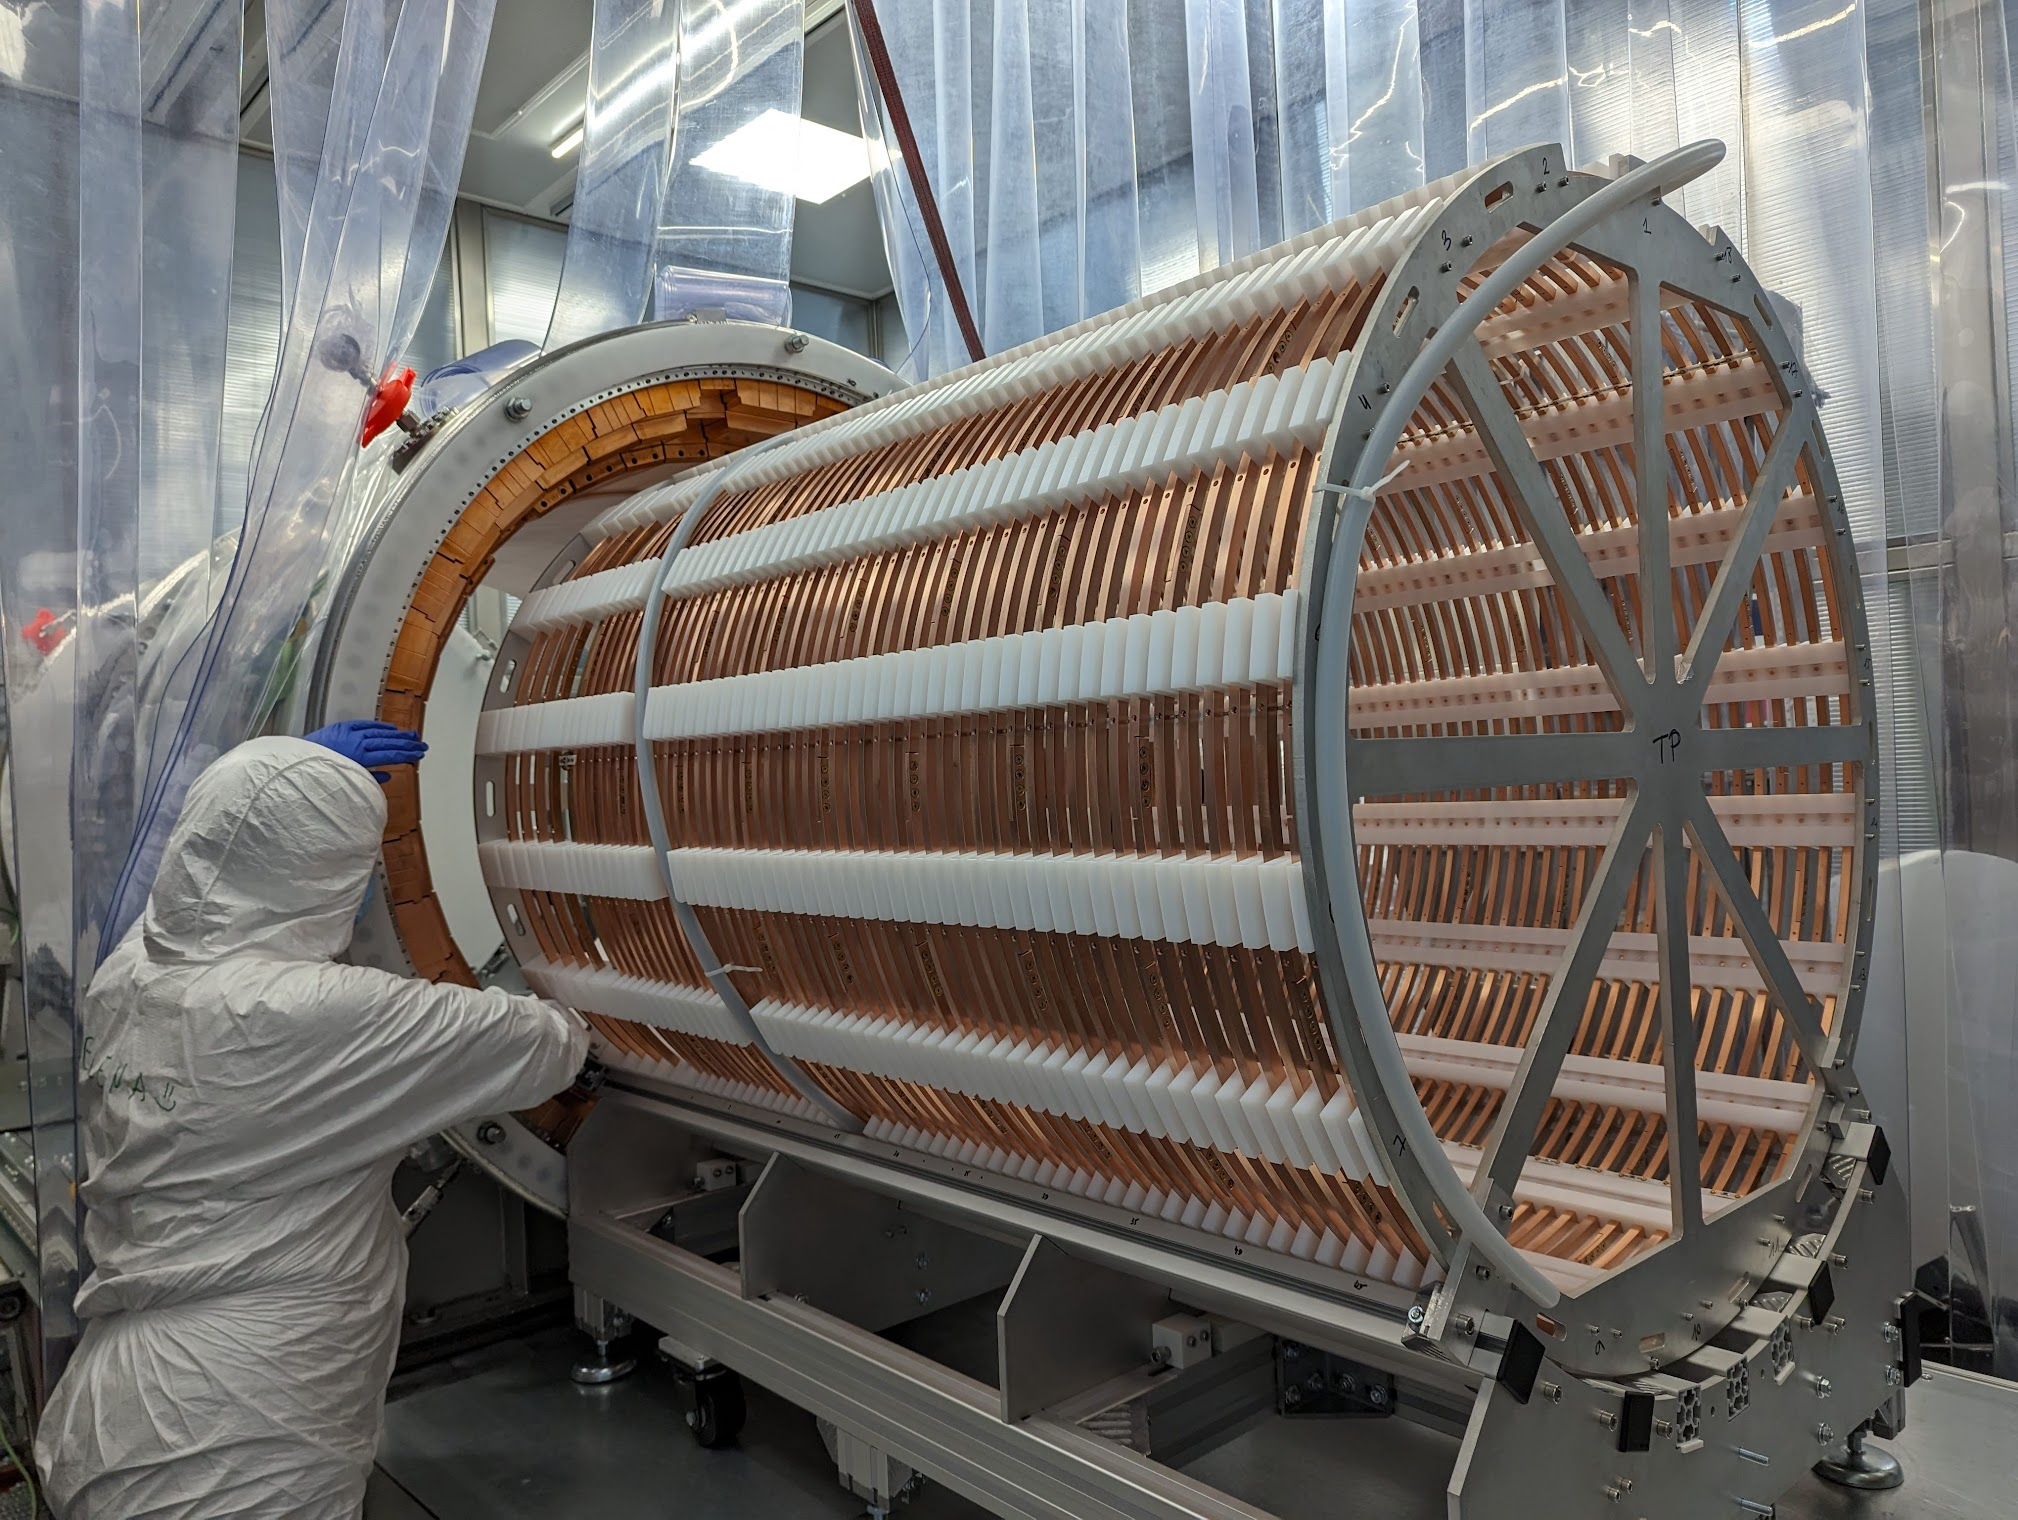
\includegraphics[width=8cm]{img/next-100-fc.jpg}
\caption{El detector NEXT, en operación actualmente en el LSC.}
\label{fig:xess}
\end{center}
\end{figure}

El experimento NEXT busca demostrar que el neutrino es su propia antipartícula mediante la detección de desintegraciones beta sin neutrinos ($\beta\beta0\nu$) que podrían producirse en el isótopo ${}^{136}$Xe del Xenón. Para ello, a lo largo de los últimos quince años, la colaboración internacional, liderada en la actualidad por el DIPC\footnote{J.J. Gómez Cadenas es el spokesperon, F. Monrabal el coordinador técnico y los coordinadores de operación son R. Soleti, H. Almazán y J. Pelegrín, todos ellos personal DIPC.} ha desarrollado una serie de cámaras de proyección temporal (TPCs) operando a alta presión. En la actualidad, el detector NEXT-100, que contiene 100 kilos de xenon enriquecido al 90\% en ${}^{136}$Xe ha entrado en operación en el LSC. Se trata de un aparato único en el mundo, cuyo principal objetivo es demostrar que la tecnología HPXe (cámaras TPC a alta presión) puede extenderse a detectores albergando masas de una tonelada. El programa NEXT incluye la operación inicial de NEXT-100 (2025-2027), seguida de una importante mejora técnica que implica la instalación de un detector de fibras óptica que permitirá una medida óptima de la energía (2027) y de la propuesta de construcción de un detector de una tonelada. Para ello se está estudiando la colaboración con el experimento KamLAND-Zen, que posee en la actualidad una tonelada de Xenón enriquecido y cuyo programa experimental concluye en 2030, fecha a partir de la cual podría construirse un futuro detector NEXT-ZEN con la tecnología demostrada por NEXT-100 y una masa total de una tonelada.  Este detector tendría un altísimo potencial de realizar un descubrimiento fundamental. 

\subsection*{Hyper-Kamiokande}

\subsection*{Física Coherente de Neutrinos}

Las tecnologías en desarrollo para los experimentos de física coherente de neutrinos son: 

\begin{enumerate}
\item El detector \xess,  una cámara de alta presión, equipada con sensores de bajo ruido que puede operar con diversos gases nobles.  
\item El detector \cess, basado en cristales monolíticos de yoduro de cesio (CsI) puro, operando a temperaturs criogénicas.
\item El detector  \gess, basado en cristales monolíticos de germanio con ruido extremadamente bajo.
\end{enumerate}

Las tres tecnologías se están desarrollando en el DIPC. En la actualidad contemplamos la instalación de \gess\ y \cess\ en una primera fase en JPARC, con una segunda fase en la ESS en la que se instalarían estos dos detectores junto a  \xess.  

\section*{El detector \xess: Diseño de base y R\&D}

\begin{figure}[bht!]
\begin{center}
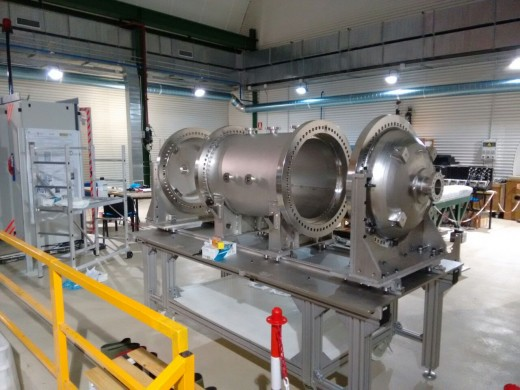
\includegraphics[width=8cm]{img/vessel2.jpg}
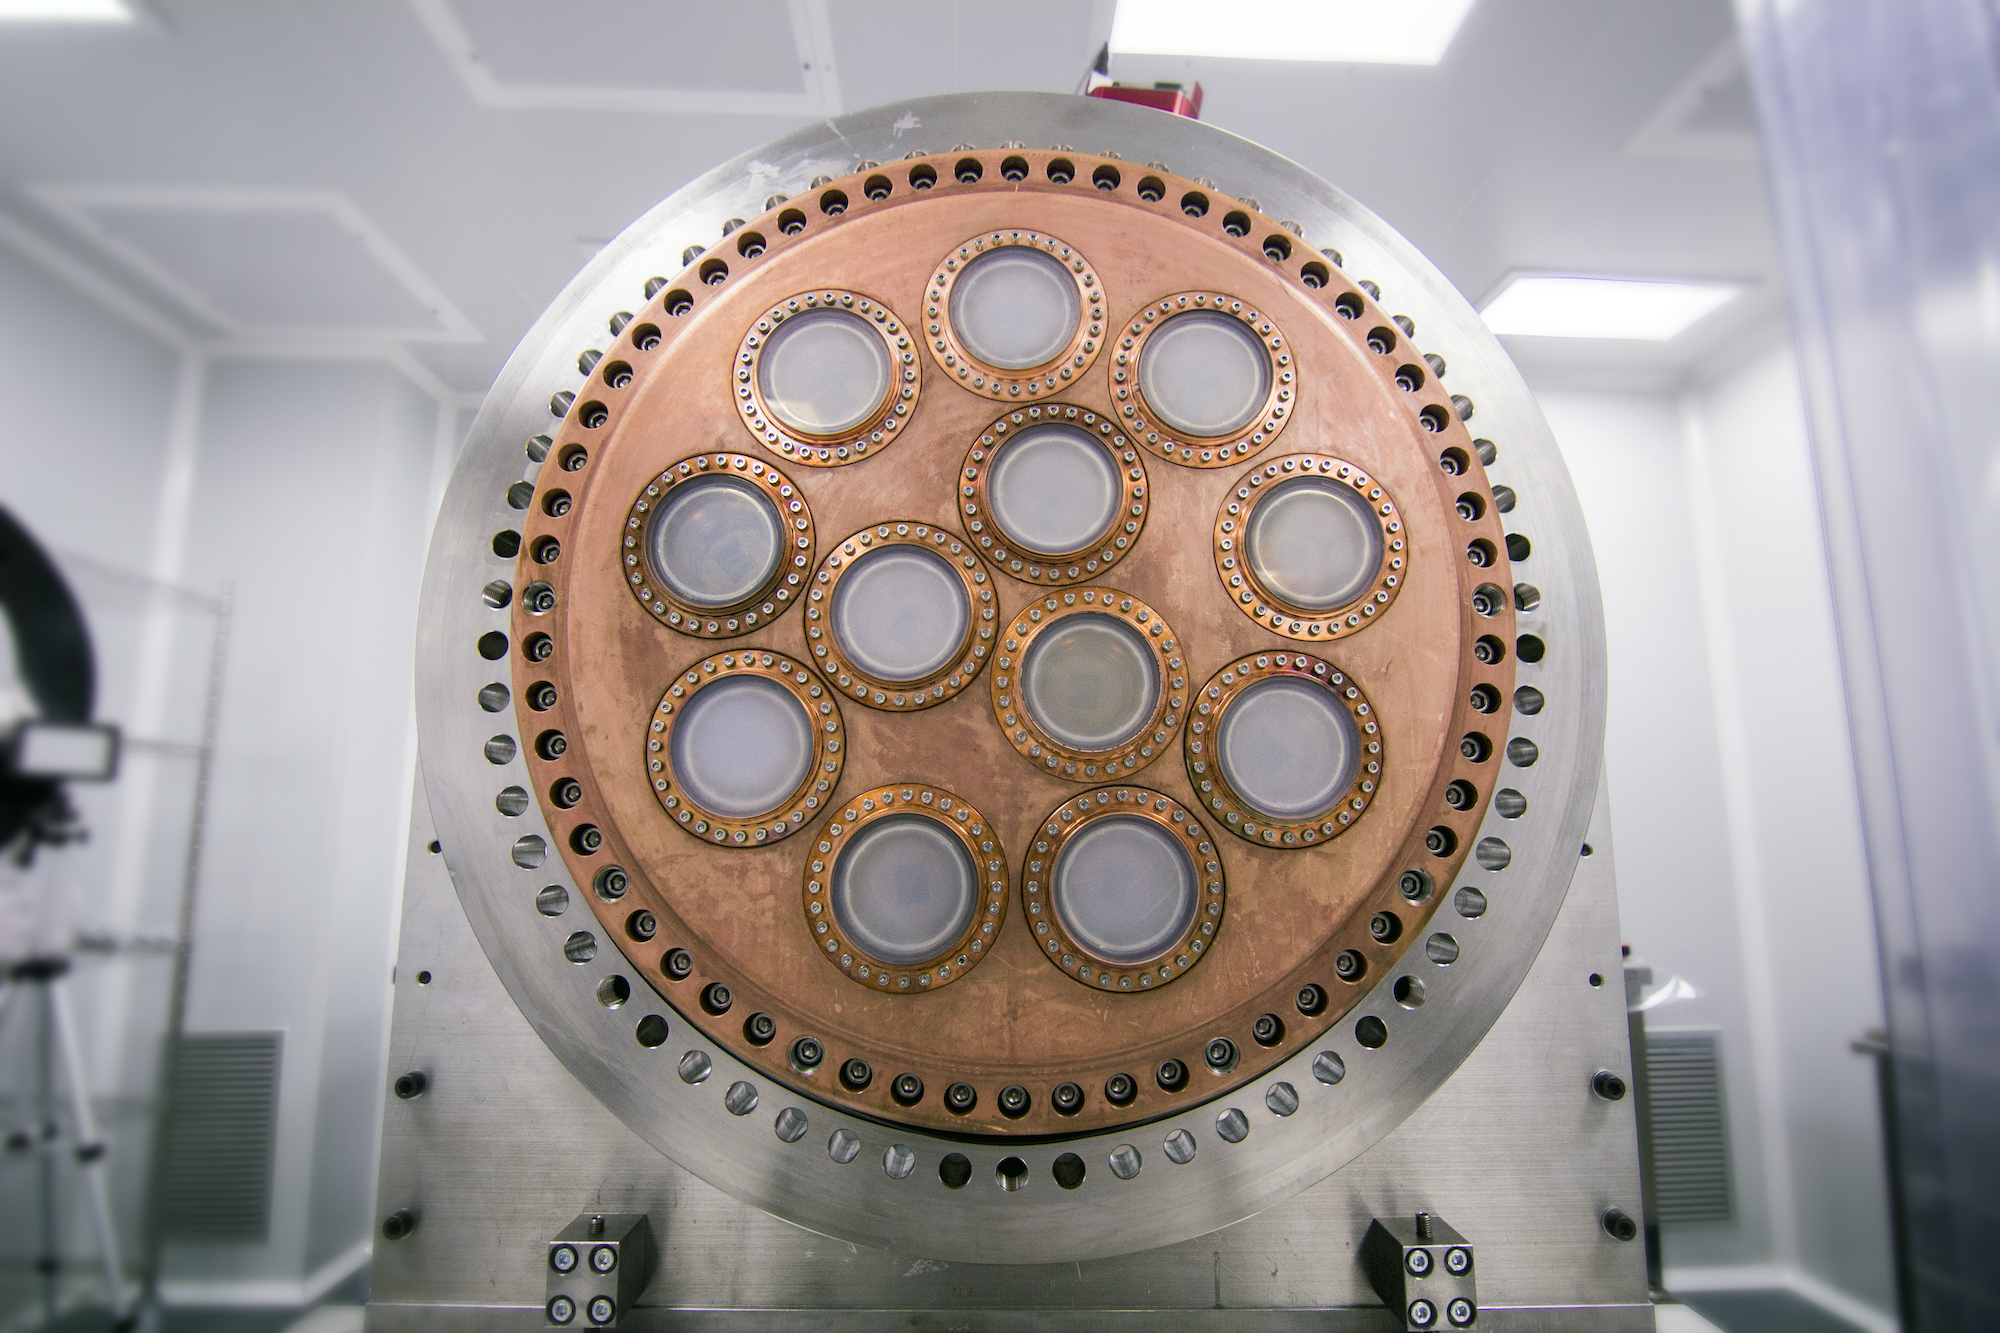
\includegraphics[width=8cm]{img/ep-new.jpg}

\caption{Arriba: vasija de presión de \xess. Abajo. Plano de PMTs}
\label{fig:xess}
\end{center}
\end{figure}

La figura \ref{fig:xess} muestra dos elementos cruciales de \xess, la cámara de presión y uno de los planos de sensores. El detector \xess\ es una cámara de proyección temporal optimizada para operar a muy alta presión (hasta 50 bares) y leída por dos planos de fotomultiplicadores (PMTs). La ventaja de este diseño es su simplicidad y robustez, así como la disponibilidad de PMTs de excelentes prestaciones (buena sensibilidad en la zona del UV donde emite el xenon y muy baja radioactividad). Un avance importante durante 2024 ha sido la recuperación del detector NEXT-White, tras completar su operación en el LSC. La vasija de alta presión de NEXT-White posee las característica apropiadas para \xess. Disponemos también de los PMTs necesarios para operar el detector, como se ilustra en la figura. 


No obstante, existe la posibilidad de mejorar la eficiencia de detección usando SiPMs (sensible al UV) o  fibras ópticas. Ambas tecnologías son parte de nuestro programa de R\&D y serán estudiadas por los prototipos \gap\ y \xed. En caso de que los resultados sean lo bastante prometedores, se introducirán dichos sensores en una segunda fase de operación de \xess. El desarrollo de la calorimetría basada en fibras ópticas es por tanto sinérgico entre el programa de física coherente de neutrinos y el programa NEXT. 


\section*{El detector \ged. Operación en la CN de Vandellós}

\begin{figure}[bht!]
\begin{center}
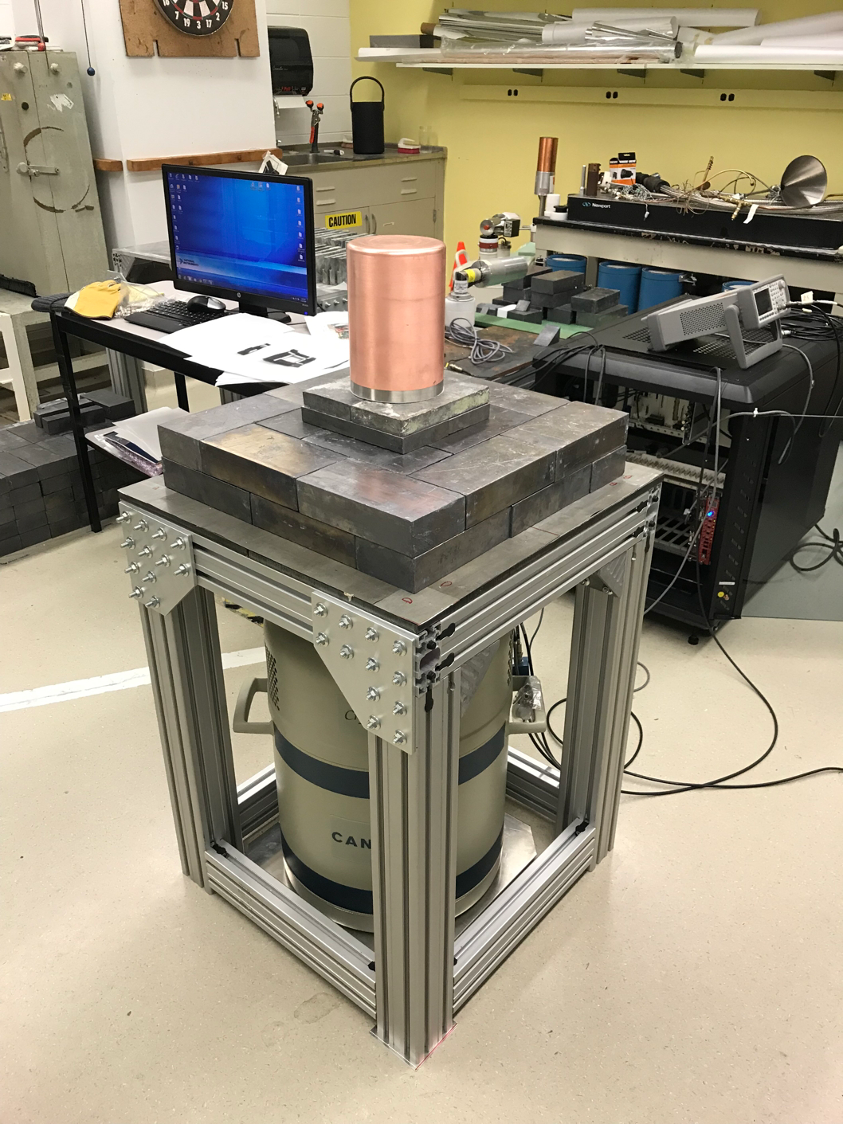
\includegraphics[width=10cm]{img/hdge.png}
\caption{El detector \ged.}
\label{fig:crysp}
\end{center}
\end{figure}

\begin{figure}[ht!]
\begin{center}
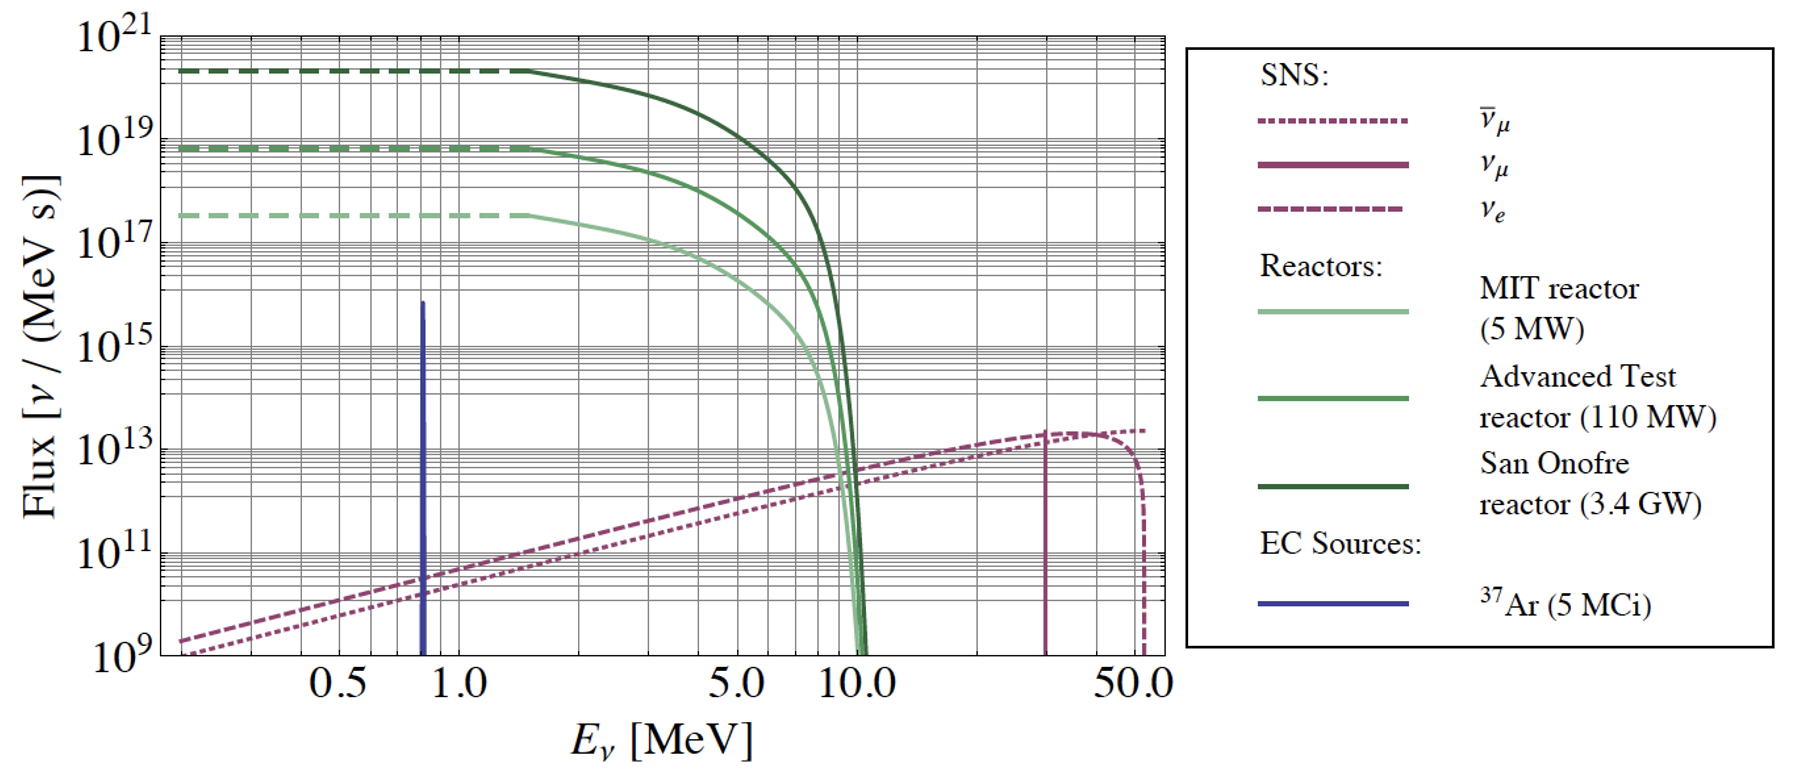
\includegraphics[width=12cm]{img/nuflux.png}
\caption{Flujos de neutrinos en reactores nucleares (líneas verdes) y en una fuente de espalación de neutrones (líneas magenta). }
\label{fig:nuflux}
\end{center}
\end{figure}

El detector \ged\ es el primer módulo completo de la tecnología \gess. Consiste en un cristal monolítico gigante de germanio ultrapuro leído por electrónica de bajísimo ruido. Se trata de un aparato único en el mundo por su umbral de detección extremadamente reducido, que permitirá medidas de gran precisión en la ESS. 
%A lo largo de 2023 se ha completado su puesta a punto y planeamos realizar una primera ronda de medidas, a lo largo de 2024, en la central nuclear de Vandellós (CNV). 


El aparato está operando en la central nuclear de Vandellós (CNV). Se trata de un hito importantísimo. Una central nuclear es una fuente intensísima de neutrinos de energías similares a los que se producen en la ESS (figura \ref{fig:nuflux}) y por tanto apropiados tanto para caracterizar los detectores como para realizar medidas de física complementarias. Por otra parte, para poder aprovechar esos neutrinos es necesario situar un detector en una posición muy cercana al reactor y a la vez muy bien blindada de los neutrones y la radioactividad que se producen allí. Se da la extraordinaria circunstancia de que la CNV posee una ``galería de tendones'' que goza exactamente de esas características.  Tras obtener el permiso de operación estamos ya tomando datos en CNV, con un programa que se extenderá a lo largo de todo el 2025. 


\section*{Progreso científico durante 2024}

A lo largo del año 2024, se han completado las siguientes tareas:
\begin{itemize}
\item Operación del Prototipo Gaseoso (\gap), primer aparato de medida para el proyecto \xess. 
\item Construcción de un criostato para operación criogénica de cristales de CsI, necesario como primer prototipo, tanto para el detector  \cess\ como para el scanner CRYSP. 
\item Construcción de un evaporador de TPB, necesario para todos los proyectos relacionados con las cámaras de xenón, ya que este emite luz ultravioleta muy dura (173 nm) que debe desplazarse mediante un cambiador molecular (tetraphenil-butiadeno, TPB) hacia longitudes de onda donde operan bien los sensores ópticos como SiPMs y PMTs (e.g, 420 nm).  
\item Preparación del primer prototipo de CRISP. 
\item Construcción del detector \xed, un aparato de escala intermedia (5 kg de xenón) que permitirá estudiar varias tecnologías para \xess.  
 
\end{itemize}

Además, se ha equipado el área experimental en Miramon,  que en la actualidad alberga los prototipos \xed\ y \ged, un taller mecánico, un taller de electrónica y el evaporador  molecular. 


\section*{Operación de \gap}
\begin{figure}[bht!]
\begin{center}
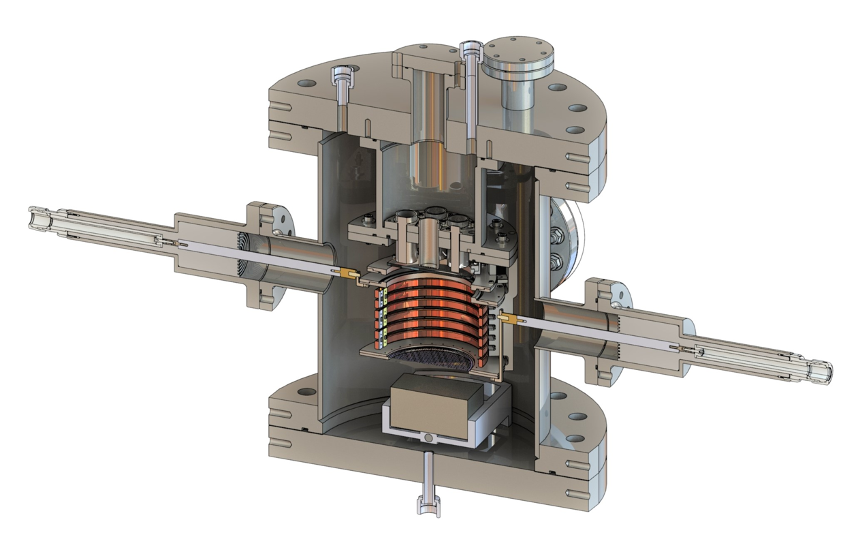
\includegraphics[width=12cm]{img/gap.png}
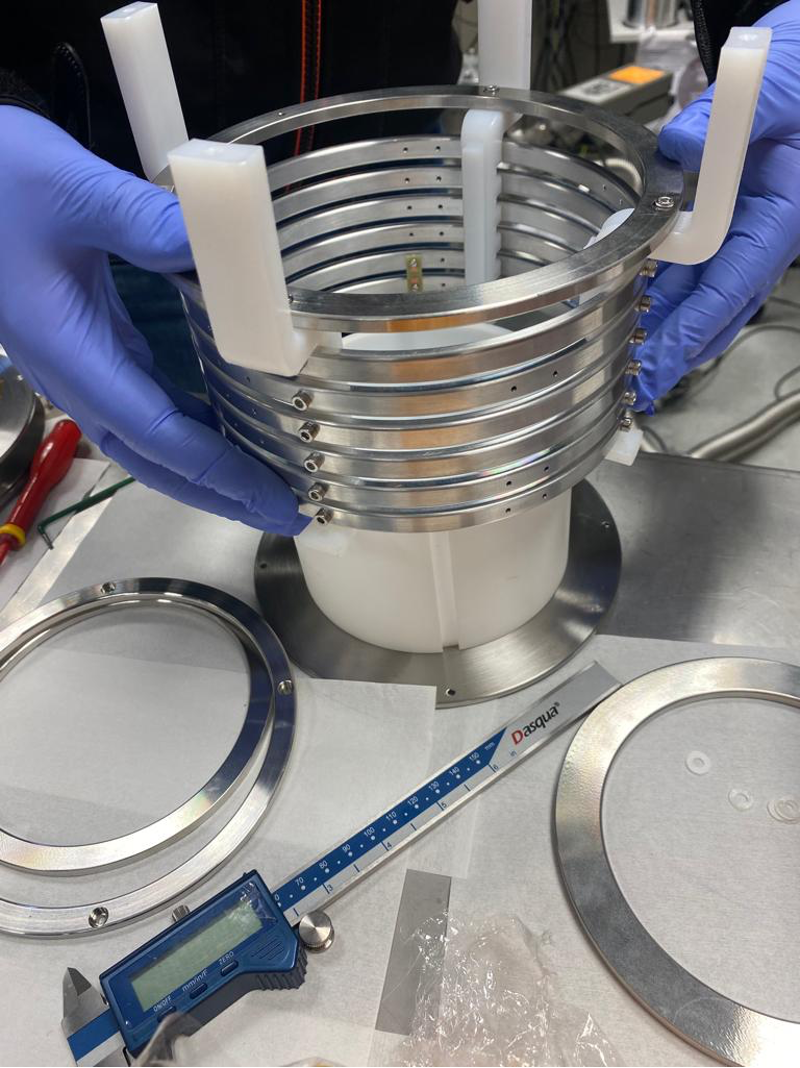
\includegraphics[width=6cm]{img/gap-fc.png}
\caption{Panel superior: diseño del detector \gap. Panel inferior: jaula eléctrica a punto de ser introducida en el detector.}
\label{fig:gap}
\end{center}
\end{figure}


\begin{figure}[bht!]
\begin{center}
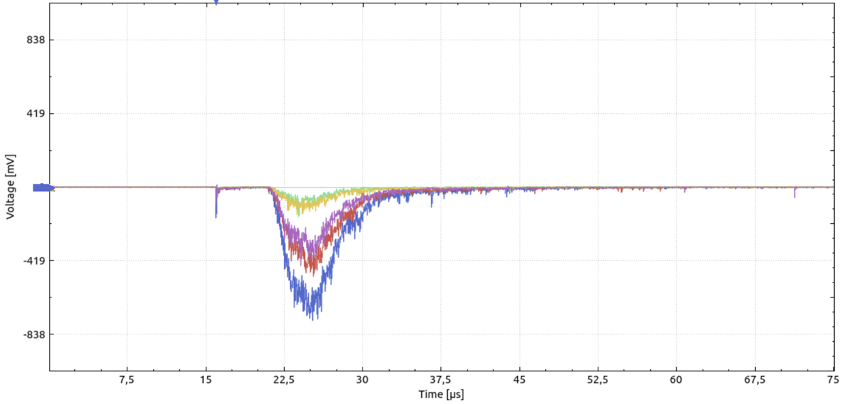
\includegraphics[width=12cm]{img/wvfm.png}
\caption{Respuesta de \gap\ a un evento de desintegración de ${}^{241}$Am (detalles en el texto).}
\label{fig:wvf}
\end{center}
\end{figure}

El detector \gap\ (figura \ref{fig:gap}) es el primer prototipo del futuro detector \xess\ (el segundo prototipo, \xed, se construirá en 2024). El objetivo de \gap\ es  caracterizar la técnica de detección coherente de neutrinos en el régimen de baja energía, ($\sim$keV), donde la señal producida por la dispersión elástica de neutrinos con núcleos as alta. El aparato es una pequeña TPC cuya región de deriva era originalmente de 2 cm (en la actualidad ha sido ampliada a 10 cm). Utiliza electroluminescencia para amplificar la señal, siendo la región de amplificación de 0.9 cm. En la primera versión del aparato, la luz producida es detectada por 7 tubos fotomultiplicadores modelo Hamamatsu R7378A. Entre la región de producción de luz y los fotosensores hay una ventana de cuarzo recubierta con tetrafenil butadieno (TPB), un cambiador de longitud onda que desplaza la luz de centelleo de los gases nobles, en el ultravioleta (170 nm), al azul (420 nm), facilitando su detección.

El detector se ha construido durante la primera mitad de 2023 y operó por primera vez en verano de ese año, con argón a 9.5 bares. Dos fuentes radiactivas, una de ${}^{83m}$Kr y otra de ${}^{241}$Am, fueron empleadas para calibrar el detector. La figura \ref{fig:wvf} muestra la respuesta típica del detector a un evento de desintegración de ${}^{241}$Am, en el que se produce una partícula alpha que interacciona en el gas, produciendo una rápida señal de electroluminescencia (S1), seguida, algunos microsegundos más tarde por una segunda señal, más intensa correspondiente a la amplificación en el ánodo (S2). En la figura se muestra la señal de 5 fotomultiplicadores diferentes. El primer pulso se corresponde con S1, mientras que el segundo pulso se corresponde S2. 

Los primeros estudios han indicado una eficiencia de colección de luz, de alrededor del 1\%. Para mejorar esa eficiencia, se han introducido una serie de mejoras en el aparato durante la segunda mitad de 2023. En concreto:
\begin{enumerate}
\item Se ha modificado la región de electroluminiscencia para evitar regiones con un campo eléctrico demasiado elevado que, al intentar operar a altos voltajes, sobrepasaba la tensión de ruptura, limitando así el voltaje de operación y, en consecuencia, la amplificación de señal.
\item Se ha añadido un tubo de teflón, recubierto con TPB, alrededor del volumen de deriva. El teflón es un magnífico reflector y permite recuperar buena parte de la luz emitida que no va dirigida a los fotosensores.
\item Se ha alargado la región de deriva hasta los 10 cm, de manera que la tasa de interacciones en el detector es mucho mayor, permitiendo discernir claramente la presencia de fuentes radiactivas.
\item Se han acercado considerablemente los sensores a la zona de amplificación para maximizar el ángulo solido de detección. Para ello se ha suprimido la ventana de cuarzo situada entre región de amplificación y fotosensores. Asimismo, los fotomultiplicadores (PMTs) han sido recubiertos directamente con TPB para aumentar la eficiencia de colección.
\end{enumerate}

La operación de \gap, incluyendo todas estas mejoras se realizará a lo largo 
del año 2024. En una segunda etapa, también en 2024, se sustituirán los PMTs for SiPMs de gran área, sensibles a la luz ultravioleta. Esto permitirá evaluar cuantitativamente las prestaciones de ambas técnicas de detección. 

\section*{Construcción y operación de \crysp}

\begin{figure}[bht!]
\begin{center}
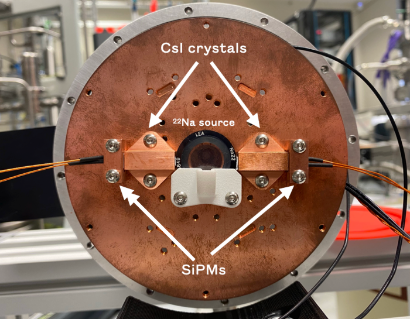
\includegraphics[width=8cm]{img/cryo0.png}
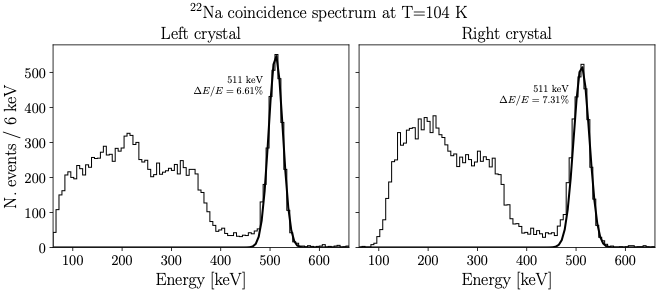
\includegraphics[width=12cm]{img/eres.png}
\caption{Izquierda: los dos detectores de CsI situados en la base del criostato, con una fuente de ${}^{22}$Na entre ambos. Derecha. Primera medida de la resolución de ambos cristales.}
\label{fig:crysp}
\end{center}
\end{figure}


El prototipo \crysp\ consiste en dos cristales de CsI, ($3\times 3 \times 20$ mm$^3$), situados frente frente en el interior de un criostato y operando a la temperatura del nitrógeno líquido. Una fuente de ${}^{22}$Na, permite medir la respuesta de ambos cristales (en coincidencia) a fotones de 511 keV (figura \ref{fig:crysp} panel izquierdo). El objetivo de este prototipo es ganar experiencia con la operación en frío de cristales de 
CsI puros y realizar una primera medida de la resolución en energía que dichos cristales pueden alcanzar (figura \ref{fig:crysp} panel derecho). La resolución en energía es del orden del 6-7\%, casi un factor 2 mejor de la resolución obtenida por cristales de LYSO (que se consideran un estándar de instrumentación). Esta excelente resolución es posible gracias a la gran luminosidad de los cristales de CsI puros en modo criogénico (del orden de 10$^5$ fotones por MeV) y permite un umbral de detección muy bajo para interacciones de neutrinos. 

El sistema se mejorará a lo largo de 2024, incorporando varias mejoras:

\begin{enumerate}
\item Se reemplazarán los pequeños cristales de \crysp\ por cristales monolíticos mucho mayores ($50 \times 50 \times 50$ mm$^3$). 
\item Se utilizarán arrays de SiPMs de mayor ganancia y electrónica rápida de bajo ruido.  
\item Se instalarán los cristales en el interior de un nuevo criostato de mejores prestaciones (aislamiento, estabilidad térmica). 
\end{enumerate}

%\section*{Construcción y operación de \ged}
%
%\begin{figure}[bht!]
%\begin{center}
%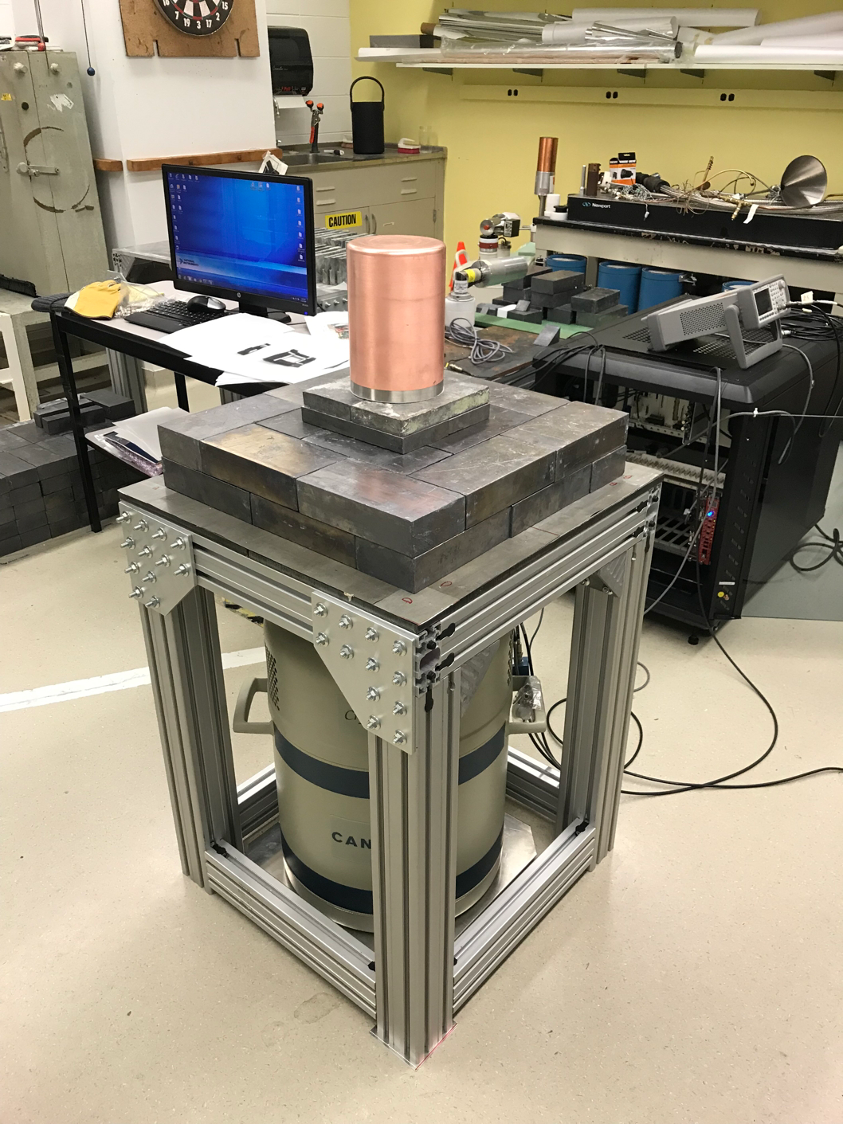
\includegraphics[width=10cm]{img/hdge.png}
%\caption{El detector \ged.}
%\label{fig:crysp}
%\end{center}
%\end{figure}
%
%\begin{figure}[ht!]
%\begin{center}
%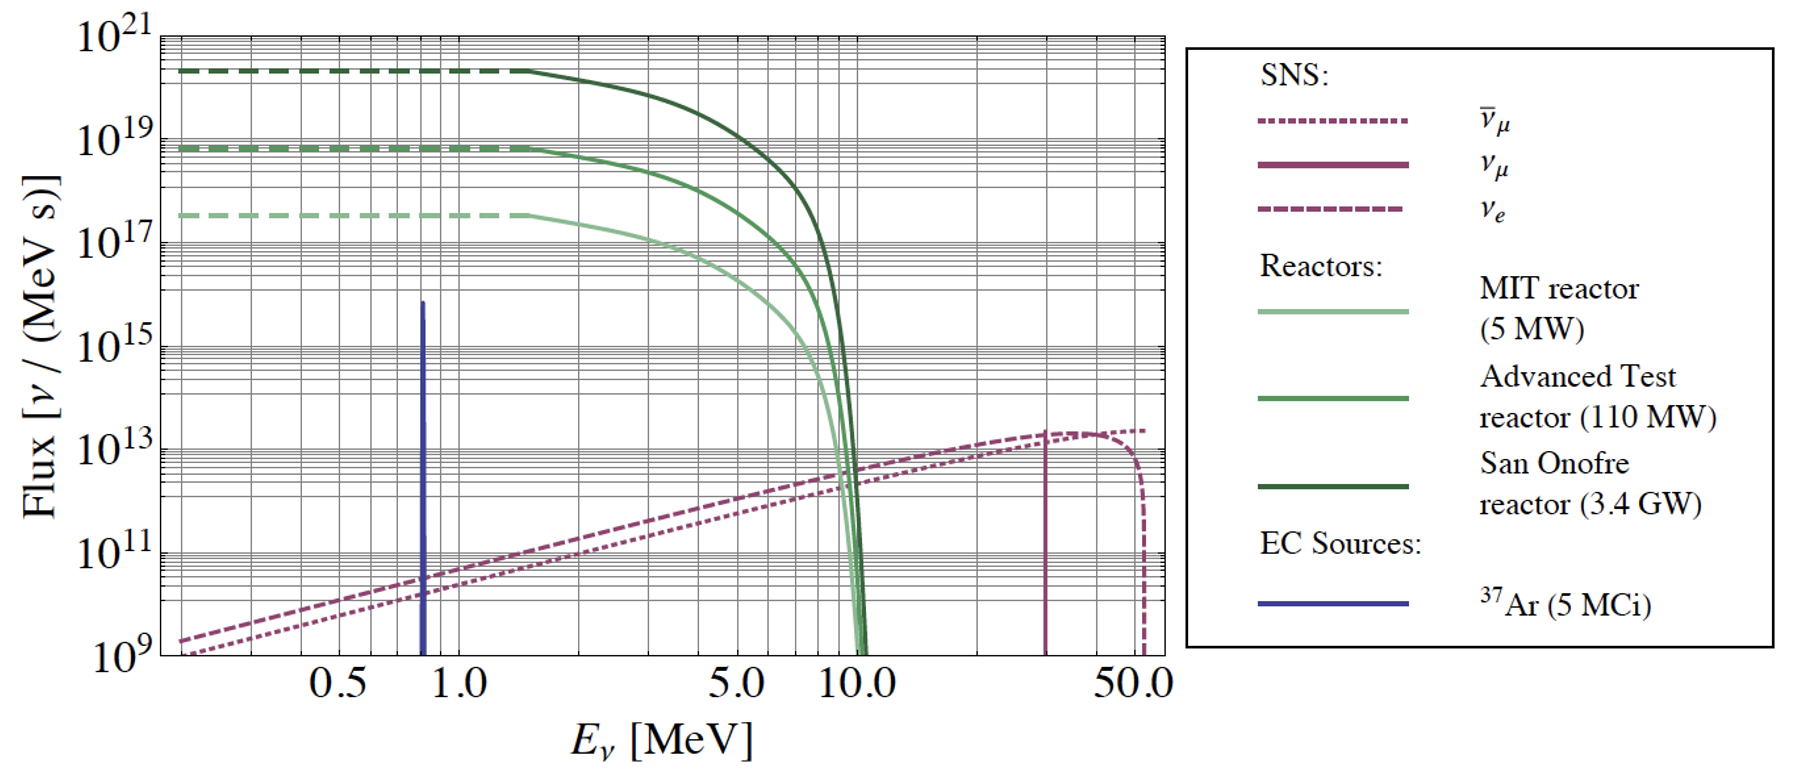
\includegraphics[width=12cm]{img/nuflux.png}
%\caption{Flujos de neutrinos en reactores nucleares (líneas verdes) y en una fuente de espalación de neutrones (líneas magenta). }
%\label{fig:nuflux}
%\end{center}
%\end{figure}
%
%El detector \ged\ consiste en un crystal monolítico gigante de germanio ultrapuro leído por electrónica de alta precisión. Se trata de un aparato único en el mundo por su umbral de detección extremadamente bajo, que permitirá medidas de gran precisión en la ESS. A lo largo de 2023 se ha completado su puesta a punto y planeamos realizar una primera ronda de medidas, a lo largo de 2024, en la central nuclear de Vandellós (CNV). 
%
%Durante el año 2023, hemos negociado el permiso para operar \ged\ en la CNV. Se trata de un hito importantísimo. Una central nuclear es una fuente intensísima de neutrinos de energías similares a los que se producen en la ESS (figura \ref{fig:nuflux}) y por tanto apropiados tanto para caracterizar los detectores como para realizar medidas de física complementarias. Por otra parte, para poder aprovechar esos neutrinos es necesario situar un detector en una posición muy cercana al reactor y a la vez muy bien blindada de los neutrones y la radioactividad que se producen allí. Se da la extraordinaria circunstancia de que la CNV posee una ``galería de tendones'' que goza exactamente de esas características y además el consejo de seguridad nuclear ha mediado para garantizar a nuestro grupo el permiso de operación. Esto nos permite, a lo largo de 2024/2025, realizar un importante programa de física, utilizando el detector \ged, antes de su operación en la ESS (a partir de 2026). 

\section*{Construcción del cryostato de CRYSP}

\section*{Construcción del evaporador}



\section*{Construcción del detector \xed}

\begin{figure}[htbp]
\begin{center}
\includegraphics[width=10cm]{img/DEMO-TPC.png}
\includegraphics[width=10cm]{img/DEMO-Fibras.png}
%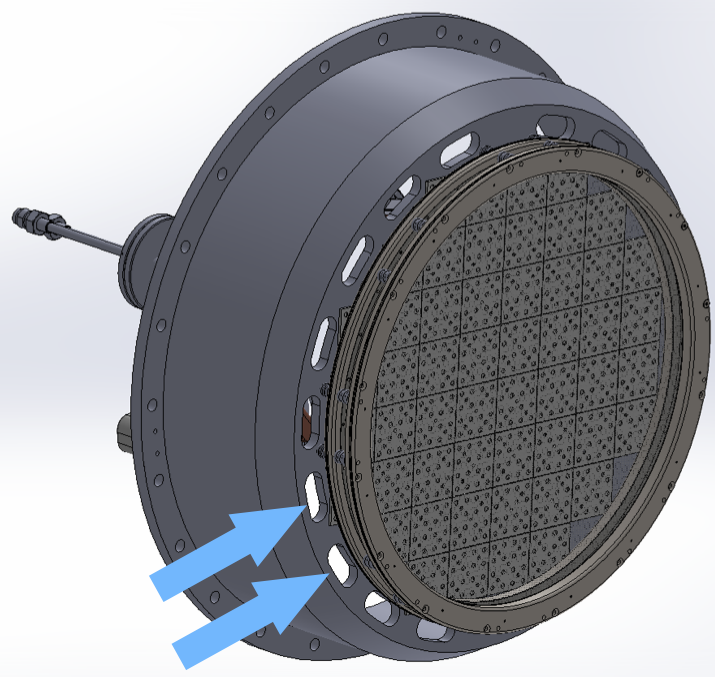
\includegraphics[width=6cm]{img/TP.png}
\caption{El detector \xed.}
\label{fig:Xe-DEMO}
\end{center}
\end{figure}

Tras el prototipo {\bf GAP}, el detector 
\xed\ permitirá escalar la tecnología de detección de neutrinos basada en cámaras de gas a un tamaño compatible con experimentos en la ESS.

La figura \ref{fig:Xe-DEMO}  muestra un esquema del detector. La vasija externa, con dimensiones de 730 mm de diámetro y 1420 mm de largo, puede resistir presiones en exceso de 20 atmósferas. La instrumentación interna divide el aparato en dos mitades simétricas. En cada una de las mitades se instala una cámara de proyección temporal (TPCs), con un cátodo común y dos ánodos simétricos ({\em field cage}). El diámetro de cada TPC es de 350 mm y su longitud es de 270 mm.  Una rejilla electroluminescente permite ampliar la señal de los electrones de deriva en cada ánodo. Los planos de detección situados detrás de cada uno de estos ({\em tracking plane}) estarán basados en SiPMs. Además, el detector incluye un barril de fibras cuyo objetivo es medir de manera uniforme la energía del evento y proporcionar un trigger. 

Las fibras ópticas, manufacturadas por Kuraray, estarán recubiertas con un transformador de longitud de onda (WLS de las siglas en inglés {\em wavelength shifter}), en nuestro caso, tetraphenyl-butiadeno (TPB). El recubrimiento de las fibras requiere la construcción de un evaporador molecular. Además la operación del aparato precisa de un sofisticado sistema de gas capaz de mantener a alta presión bajo condiciones de extrema estanqueidad y limpieza, los 5 kilos de gas xenón que el aparato puede contener. 

A lo largo de 2023 se ha completado casi totalmente el diseño del aparato que será construido en 2024 y se han adquirido una parte de las componentes necesarias (infraestructuras), tal como se describe más abajo.  

\section*{Colaboraciones estratégicas}

Además de las colaboraciones estratégicas ya iniciadas (con TEKNIKER, CEIT y AVS), a lo largo de 2023 se ha iniciado una importante colaboración con LIPP (Lisboa), que ha tomado la responsabilidad de cortar y aluminizar las fibras para el detector \xed\ que se construirá en 2024. Además, estamos explorando un proyecto conjunto con FAGOR para  
desarrollar diodos de avalancha (APDs) de gran área para el proyecto \cess.  
 

\section*{Justificación del presupuesto concedido en 2024}

Se justifica un presupuesto de 500,000 \euro, distribuido en los siguientes bloques: a) personal; b) viajes y formación; c) acuerdos de colaboración (LIPP);  d) sensores para \xess; e) material de laboratorio e informática, f) evaporador molecular y g) construcción de prototipos. 

 \subsection*{a. Personal}
 
 El grupo de neutrinos del DIPC consiste en la actualidad de veinticinco miembros. Dos profesores Ikerbasque (Collar y Gómez-Cadenas), dos asociados Ikerbasque (Ferrario y Monrabal), dos físicos senior (López y Zerzion), dos asociados post-doctorales senior (Soleti y Simó), cinco asociados post-doctorales junior (Aramburu, Brodolin, Barcelón, Torelli y Lewis), cinco estudiantes de doctorado (Valle, Yubero, Elorza, Barrio-Torregrosa y Seeman), cuatro ingenieros mecánicos (Oblak, Castillo, Taboada y Torrent), un ingeniero electrónico (Dietz) un ingeniero criogénico (Pelegrín) y un técnico electrónico (Echevarría). Los salarios de la mayor parte de este personal son cubiertos por Ikerbasque, DIPC, IKUR y los tres proyectos ERC mencionados más arriba. 
 
 En 2023 este proyecto ha financiado el salario de  Oblak (12 meses), el salario de Pelegrín (3 meses) y el salario de Zerzión (10 meses). 
 
 \begin{table}[h!]
\caption{\large{\textbf{Nóminas 2023}}}
\begin{center}
\begin{tabular}{p{0.50\linewidth}   r }%p{0.25\linewidth} r}

\textbf{Concepto}&\makecell[l]{ \textbf{Cantidad} } \\ \\  \hline\hline
\\
{\footnotesize {Oblak  }}&{\footnotesize {51,811 \euro{} }}  \\ 
{\footnotesize {Pelegrín}}&{\footnotesize {12,333 \euro{} }} \\
{\footnotesize {Zerzión}}&{\footnotesize {53,509 \euro{} }}  \\ 

\makecell[l] {\textbf{Personal}}&\textbf{117,653 \euro{}}  \\  \\ \hline \hline 
\end{tabular}
\end{center}
\label{personel2024}
\end{table}%
 
\subsection*{b. Viajes y formación}
  
  A lo largo del año se han realizado un cierto número de viajes, para visitas a empresas y otros centros de investigación, así como actividades de formación.  
  
 \begin{table}[h!]
\caption{\large{\textbf{Viajes y formación 2023}}}
\begin{center}
\begin{tabular}{p{0.50\linewidth}   r }%p{0.25\linewidth} r}

\textbf{Concepto}&\makecell[l]{ \textbf{Cantidad} } \\ \\  \hline\hline
\\
{\footnotesize {Viajes }}&{\footnotesize {10,521 \euro{} }}  \\ 
{\footnotesize {Formación}}&{\footnotesize {1,380 \euro{} }} \\

\makecell[l] {\textbf{Viajes y formación}}&\textbf{11,901 \euro{}}  \\  \\ \hline \hline 
\end{tabular}
\end{center}
\label{viajes2024}
\end{table}%

\subsection*{c. Acuerdos de colaboración (LIPP)}
  
 El acuerdo de colaboración con LIPP estipula un pago único de 50,000 \euro\ por parte del DIPC, como compensación por los servicios de medida, corte, aluminizado y pruebas de calidad de las fibras ópticas para los detectores de \xess.   
 
 \begin{table}[h!]
\caption{\large{\textbf{Colaboración con LIPP 2023}}}
\begin{center}
\begin{tabular}{p{0.50\linewidth}   r }%p{0.25\linewidth} r}

\textbf{Concepto}&\makecell[l]{ \textbf{Cantidad} } \\ \\  \hline\hline
\\

\makecell[l] {\textbf{Compensación económica}}&\textbf{50,000 \euro{}}  \\  \\ \hline \hline 
\end{tabular}
\end{center}
\label{viajes2024}
\end{table}%


\subsection*{d. Adquisición de sensores para \xess}
  
 En 2023 se han adquirido 50 PMTs de altas prestaciones (operación en la zona VUV, alto rendimiento cuántico y bajo ruido), manufacturados por Hamamatsu. Se trata de los sensores que instrumentarán la primera fase del detector \xess (figura \ref{fig:xess}).   
 
 \begin{table}[h!]
\caption{\large{\textbf{Sensores para \xess}}}
\begin{center}
\begin{tabular}{p{0.50\linewidth}   r }%p{0.25\linewidth} r}

\textbf{Concepto}&\makecell[l]{ \textbf{Cantidad} } \\ \\  \hline\hline
\\

\makecell[l] {\textbf{Sensores \xess}}&\textbf{92,154 \euro{}}  \\  \\ \hline \hline 
\end{tabular}
\end{center}
\label{viajes2024}
\end{table}%

\subsection*{e. Material de laboratorio e informática}

A lo largo de 2023 se ha realizado una importante inversión para equipar la nueva área experimental de Miramon que incluye un pequeño taller mecánico para la construcción rápida de piezas para los detectores, así como componentes electrónicas (resistencias, condensadores, etc.) pequeños aparatos de medida, equipamiento de sala limpia, pequeño material informático y licencias de software. 

\begin{table}[h!]
\caption{\large{\textbf{Taller y herramientas}}}
\begin{center}
\begin{tabular}{p{0.50\linewidth}   r }%p{0.25\linewidth} r}

\textbf{Concepto}&\makecell[l]{ \textbf{Cantidad} } \\ \\  \hline\hline
\\

{\footnotesize {EPIs }}&{\footnotesize {554 \euro{} }}  \\ 
{\footnotesize {Herramientas y consumibles}}&{\footnotesize {8,546 \euro{} }}  \\
{\footnotesize {Máquinas taller (torno, fresadora, CNC)}}&{\footnotesize {24,002 \euro{} }}  \\ 
 
\makecell[l] {\textbf{Taller y herramientas}}&\textbf{33,102 \euro{}}  \\  \\ \hline \hline 
\end{tabular}
\end{center}
\label{lab2024}
\end{table}%

\begin{table}[h!]
\caption{\large{\textbf{Electrónica e informática}}}
\begin{center}
\begin{tabular}{p{0.50\linewidth}   r }%p{0.25\linewidth} r}

\textbf{Concepto}&\makecell[l]{ \textbf{Cantidad} } \\ \\  \hline\hline
\\
{\footnotesize {Componentes electrónicos }}&{\footnotesize {1,724 \euro{} }}  \\ 
{\footnotesize {Informática: licencias y hardware}}&{\footnotesize {28,372 \euro{} }}  \\ 

\makecell[l] {\textbf{Electrónica e informática}}&\textbf{30,096 \euro{}}  \\  \\ \hline \hline 
\end{tabular}
\end{center}
\label{lab2024}
\end{table}%

\subsection*{f. Evaporador molecular}

\begin{table}[h!]
\caption{\large{\textbf{Evaporador molecular}}}
\begin{center}
\begin{tabular}{p{0.50\linewidth}   r }%p{0.25\linewidth} r}

\textbf{Concepto}&\makecell[l]{ \textbf{Cantidad} } \\ \\  \hline\hline
\\
{\footnotesize {Bombas de vacío }}&{\footnotesize {32,471 \euro{} }}  \\ 
{\footnotesize {Juntas de vacío}}&{\footnotesize {145 \euro{} }}  \\ 
{\footnotesize {Fuente de alto voltaje}}&{\footnotesize {9,523 \euro{} }}  \\
{\footnotesize {SAI}}&{\footnotesize {6,779 \euro{} }}  \\ 
{\footnotesize {Sistema de Plasma}}&{\footnotesize {13,796 \euro{} }}  \\ 
\makecell[l] {\textbf{Evaporador Molecular}}&\textbf{62,714 \euro{}}  \\  \\ \hline \hline 
\end{tabular}
\end{center}
\label{lab2024}
\end{table}%

\subsection*{g. Construcción de prototipos}

\subsection*{Infraestructuras, consumibles y equipos para laboratorio}
 
 El equipamiento de los laboratorios incluye la construcción de una mesa óptica equipada con una caja negra y una prensa, así como la adquisición de productos químicos necesarios para limpieza de piezas (agua destilada, alcohol, ácido nítrico), gases, abrazaderas,  válvulas, juntas, tornillería y otros consumibles. También se han comprado los elementos necesarios para construir una tienda limpia en cuyo interior operará el detector \xed\ y piezas necesarias para la mejora de \gap\ y la construcción del criostato de \crysp. 
 
 
 \begin{table}[h!]
\caption{\large{\textbf{Laboratorios}}}
\begin{center}
\begin{tabular}{p{0.50\linewidth}   r }%p{0.25\linewidth} r}

\textbf{Concepto}&\makecell[l]{ \textbf{Cantidad} } \\ \\  \hline\hline
\\
{\footnotesize {Equipamiento laboratorio y consumibles }}&{\footnotesize {12,552 \euro{} }}  \\ 
{\footnotesize {Tienda limpia}}&{\footnotesize {9,251 \euro{} }} \\

\makecell[l] {\textbf{Total Laboratorios}}&\textbf{21,803 \euro{}}  \\  \\ \hline \hline 
\end{tabular}
\end{center}
\label{lab2024}
\end{table}%
 
 \begin{table}[h!]
\caption{\large{\textbf{\gap\ y preparación \xed}}}
\begin{center}
\begin{tabular}{p{0.50\linewidth}   r }%p{0.25\linewidth} r}

\textbf{Concepto}&\makecell[l]{ \textbf{Cantidad} } \\ \\  \hline\hline
\\
{\footnotesize {SiPMs (\gap)}}&{\footnotesize {14,142 \euro{} }} \\
{\footnotesize {Fuentes radioactivas}}&{\footnotesize {5,747 \euro{} }} \\
{\footnotesize {Paneles de fibras (prototipos)}}&{\footnotesize {1,440 \euro{} }}  \\ 
{\footnotesize {piezas jaula eléctrica}}&{\footnotesize {5,301 \euro{} }} \\
{\footnotesize {Estructura de anillos de cobre, TPC}}&{\footnotesize {39,906 \euro{} }}  \\ 

\makecell[l] {\textbf{\gap\ y  \xed}}&\textbf{66,536 \euro{}}  \\  \\ \hline \hline 
\end{tabular}
\end{center}
\label{xed2024}
\end{table}%

 \begin{table}[h!]
\caption{\large{\textbf{\crysp\ y preparación \ced}}}
\begin{center}
\begin{tabular}{p{0.50\linewidth}   r }%p{0.25\linewidth} r}

\textbf{Concepto}&\makecell[l]{ \textbf{Cantidad} } \\ \\  \hline\hline
\\
{\footnotesize {Cryostato (\crysp) }}&{\footnotesize {3,876 \euro{} }}  \\
{\footnotesize {Cristales CsI (\crysp) }}&{\footnotesize {956 \euro{} }}  \\ 
{\footnotesize {Cristales CsI (Tl) (\ced)}}&{\footnotesize {8,449 \euro{} }} \\
{\footnotesize {Electrónica \crysp}}&{\footnotesize {1348 \euro{} }}  \\ 

\makecell[l] {\textbf{Total \xed}}&\textbf{14,629 \euro{}}  \\  \\ \hline \hline 
\end{tabular}
\end{center}
\label{ced2024}
\end{table}

\subsection*{Presupuesto total}

Los gastos totales ascienden a 500,588 \euro. Se justifican 500,000 \euro. 

 \begin{table}[h!]
\caption{\large{\textbf{Justificación financiación 2023}}}
\begin{center}
\begin{tabular}{p{0.50\linewidth}   r }%p{0.25\linewidth} r}

\textbf{Concepto}&\makecell[l]{ \textbf{Cantidad} } \\ \\  \hline\hline
\\
{\footnotesize {Personal }}&{\footnotesize {117,653 \euro{} }}  \\ 
{\footnotesize {Viajes y formación}}&{\footnotesize {11,901 \euro{} }} \\
{\footnotesize {Acuerdos de colaboración}}&{\footnotesize {50,000 \euro{} }} \\
{\footnotesize {PMTs para \xess}}&{\footnotesize {92,154 \euro{} }} \\
{\footnotesize {Taller y herramientas}}&{\footnotesize {33,102 \euro{} }} \\
{\footnotesize {Electrónica e informática}}&{\footnotesize {30,0965 \euro{} }} \\
{\footnotesize {Equipamiento de laboratorio}}&{\footnotesize {21,803 \euro{} }}  \\
{\footnotesize {Evaporador molecular}}&{\footnotesize {62,714 \euro{} }}  \\ 
{\footnotesize \gap\ y \xed}&{\footnotesize {66,536 \euro{} }}  \\ 
{\footnotesize \crysp\ y \ced}&{\footnotesize {14,629 \euro{} }}  \\ 
\makecell[l] {\textbf{Total}}&\textbf{500,588 \euro{}}  \\  \\ \hline \hline 
\end{tabular}
\end{center}
\label{tot2024}
\end{table}
\end{document}